\documentclass[a4paper,12pt]{article}
\usepackage[a4paper]{geometry}
\usepackage{color, hyperref}
\usepackage[hypcap]{caption}
\usepackage[utf8]{inputenc}
\usepackage{float}
\usepackage{array}
\usepackage{ulem}
\usepackage{contour}
\usepackage{listings}
\usepackage{booktabs}
\usepackage{multirow}
\usepackage{wrapfig, graphicx}

\graphicspath{{./img}}
\hypersetup{
	colorlinks=true,
	breaklinks=true,
	linkcolor=black,
	pdftitle={PolyMessages - Sprint 1}
}

\definecolor{codegreen}{rgb}{0,0.6,0}
\definecolor{codegray}{rgb}{0.5,0.5,0.5}
\definecolor{codepurple}{rgb}{0.58,0,0.82}
\definecolor{backcolour}{rgb}{0.9,0.9,0.9}
\lstdefinestyle{myStyle}{
	backgroundcolor=\color{backcolour},
	commentstyle=\color{codegreen},
	keywordstyle=\color{magenta},
	numberstyle=\tiny\color{codegray},
	stringstyle=\color{codepurple},
	basicstyle=\ttfamily\footnotesize,
	breakatwhitespace=false,
	breaklines=true,
	captionpos=b,
	keepspaces=true,
	showspaces=false,
	showstringspaces=false,
	showtabs=false,
	tabsize=2,
	linewidth=0.8\linewidth,
	xleftmargin=0.2\linewidth,
	% padding=5px
}

\lstset{style=myStyle}


\renewcommand{\ULdepth}{1.8pt}
\contourlength{0.8pt}

\newcommand{\ul}[1]{%
	\uline{\phantom{#1}}%
	\llap{\contour{white}{#1}}%
}

\captionsetup{labelfont={it, bf}, textfont={it}}

\title{PolyMessages | Sprint 1}
\author{Eri Agnese, Marvin Bontemps, Lucas Nouguier}
\date{17 Avril 2022}

\begin{document}
\maketitle
\tableofcontents
\clearpage
\hypersetup{linkcolor=red}

\newgeometry{left=2cm,right=2cm,bottom=2cm, top=1.5cm}

\section{Protocole de communication}
\begin{figure}[h]
	\centering
	\hrulefill\\
	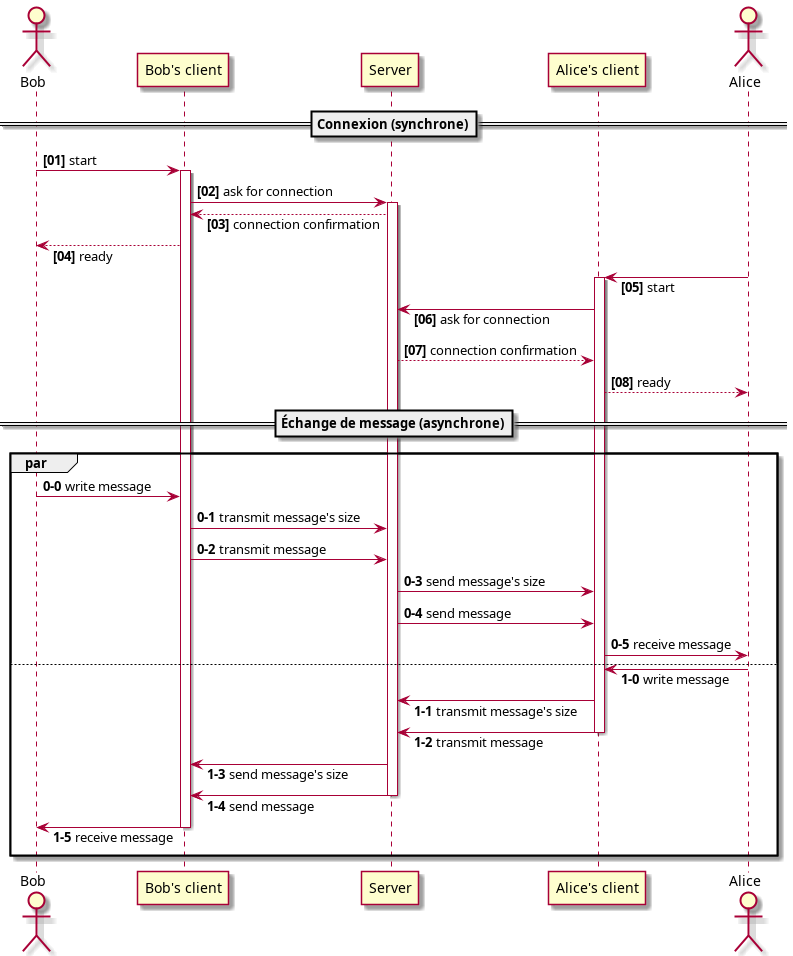
\includegraphics[width=0.925\linewidth]{sequence.png}
	\caption{Protocole de communication clients/serveur}
	\hrulefill
\end{figure}

\pagebreak
\section{Architecture}
\begin{figure}[h]
	\centering
	\hrulefill\\
	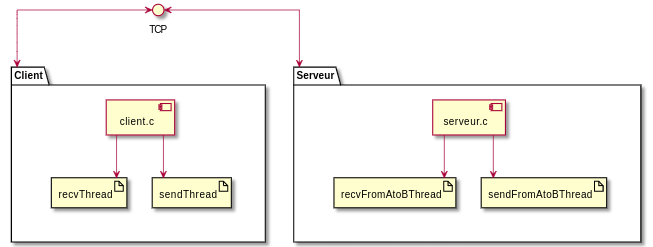
\includegraphics[width=\linewidth]{architecture.png}
	\caption{Architecture de la messagerie}
	\hrulefill
\end{figure}
\section{Répartition du travail}
\begin{wraptable}{r}{0.5\linewidth}
	\vspace{-0.5cm}
	\begin{tabular}{cccc}
		\toprule
		\multirow{2}{*}{Tâches} & \multicolumn{3}{c}{Étudiants}\\
		& Lucas & Éri & Marvin\\
		\midrule
		Initialisation & X\\
		\midrule
		Threading client & & X\\
		\midrule
		Threading serveur & & &X\\
		\midrule
		Fusion & X\\
		\bottomrule
	\end{tabular}
	\caption{Tâche effecutée par étudiant}
	\label{table:repartition}
	\vspace{-1.5cm}
\end{wraptable}
Au lancement du projet, une messagerie basique au tour par tour a été montée par Lucas car il était impossible de travailler de manière efficiente à plusieurs sur une seule fonctionnalité. Une fois cette base complète, il était possible de travailler en parallèle donc le threading du serveur et des clients ont respectivement été fait par Marvin et Éri (voir \ul{Table.~\ref{table:repartition}} \& \ul{Fig.~\ref{fig:gantt}}). La fusion de ces 2 travaux asynchrones a été effectuée par Lucas.
\begin{figure}[h]
	\centering
	\hrulefill\\
	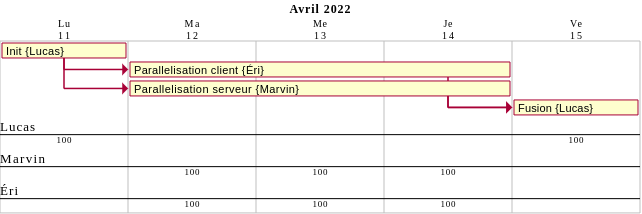
\includegraphics[width=\linewidth]{gantt.png}\\
	\caption{Diagramme de Gantt sur la réalisation du projet}
	\label{fig:gantt}
	\hrulefill
\end{figure}
\pagebreak
\section{Exécution du code}
Pour lancer la messagerie, il faut commencer par compiler et lancer le serveur
\begin{figure}[h]
	\centering
	\vspace{-0.1cm}
	\begin{lstlisting}[language=bash, gobble=4]
		[lucas@xps-lucas ~]$ gcc -o server serveur.c
		[lucas@xps-lucas ~]$ ./server <PORT>
	\end{lstlisting}
\end{figure}

\noindent On peut alors lancer les clients (actuellement il en faut 2 avant qu'un échange puisse avoir lieu)
\begin{figure}[h]
	\centering
	\vspace{-0.2cm}
	\begin{lstlisting}[language=bash, gobble=4]
		[lucas@xps-lucas ~]$ gcc -o client client.c
		[lucas@xps-lucas ~]$ ./client <IP> <PORT>
	\end{lstlisting}
\end{figure}
\section{Difficultés}
Les difficultés rencontrées ont principalement été d'ordre technique. En parler entre nous ou avec les autres nous a permis de résoudre les problèmes.
\end{document}